% ANUfinalexam.tex (Version 2.0)
% ===============================================================================
% Australian National University Final Exam LaTeX template.
% 2004; 2009, Timothy Kam, ANU School of Economics
% Licence type: Free as defined in the GNU General Public Licence: http://www.gnu.org/licenses/gpl.html

\documentclass[a4paper,12pt,fleqn]{article}
\setlength{\parindent}{0em}
\usepackage{amsmath}
\usepackage{fancyhdr}
\usepackage{siunitx}
\usepackage{enumitem}
\usepackage{amsmath}
\usepackage{graphicx}
\usepackage{tikz}
\usepackage{import}
\usepackage{comment}

% Unit definitions %%%%%%%%%%%%%%%%%%%%%%%%%%%%%%%%%%

\DeclareSIUnit\kilowatthour{kWh}
\DeclareSIUnit\kilowattpeak{kW_P}
\DeclareSIUnit\kVA{kVA}
\DeclareSIUnit\kVAR{kVAR}
\DeclareSIUnit\year{y}
\DeclareSIUnit\north{N}
\DeclareSIUnit\south{S}
\DeclareSIUnit\second{s}


% Insert your course information here %%%%%%%%%%%%%%%%%%%%%%%%%%%%%%%%%%

\newcommand{\institution}{CORNWALL COLLEGE}
\newcommand{\titlehd}{BSc Renewable Energy and Carbon Management}
\newcommand{\examtype}{Exam}
\newcommand{\examdate}{Academic Year 2014-2015}
\newcommand{\examcode}{CORC2103}
\newcommand{\examtitle}{Geothermal Energy}
\newcommand{\readtime}{15 Minutes}
\newcommand{\writetime}{Two Hours}
\newcommand{\materials}{Non-programmable Calculators; Formula Sheet}
\newcommand{\middlewords}{Exam continues on next page}
\newcommand{\lastwords}{End of Exam}

%%%%%%%%%%%%%%%%%%%%%%%%%%%%%%%%%%%%%%%%%%%%%%%%%%%%

%\setcounter{MaxMatrixCols}{10}
\newtheorem{theorem}{Theorem}
\newtheorem{acknowledgement}[theorem]{Acknowledgement}
\newtheorem{algorithm}[theorem]{Algorithm}
\newtheorem{axiom}[theorem]{Axiom}
\newtheorem{case}[theorem]{Case}
\newtheorem{claim}[theorem]{Claim}
\newtheorem{conclusion}[theorem]{Conclusion}
\newtheorem{condition}[theorem]{Condition}
\newtheorem{conjecture}[theorem]{Conjecture}
\newtheorem{corollary}[theorem]{Corollary}
\newtheorem{criterion}[theorem]{Criterion}
\newtheorem{definition}[theorem]{Definition}
\newtheorem{example}[theorem]{Example}
\newtheorem{exercise}[theorem]{Exercise}
\newtheorem{lemma}[theorem]{Lemma}
\newtheorem{notation}[theorem]{Notation}
\newtheorem{problem}[theorem]{Problem}
\newtheorem{proposition}[theorem]{Proposition}
\newtheorem{remark}[theorem]{Remark}
\newtheorem{solution}[theorem]{Solution}
\newtheorem{summary}[theorem]{Summary}
\newenvironment{proof}[1][Proof]{\noindent\textbf{#1.} }{\ \rule{0.5em}{0.5em}}

% ANU Exams Office mandated margins and footer style
\setlength{\topmargin}{0cm}
\setlength{\textheight}{9.25in}
\setlength{\oddsidemargin}{0.0in}
\setlength{\evensidemargin}{0.0in}
\setlength{\textwidth}{16cm}
\pagestyle{fancy}
\lhead{} 
\chead{} 
\rhead{} 
\lfoot{} 
\cfoot{\footnotesize{Page \thepage \ of \pageref{finalpage} -- \titlehd \ (\examcode)}} 
\rfoot{} 

% DEPRECATED: ANU Exams Office mandated margins and footer style
%\setlength{\topmargin}{0cm}
%\setlength{\textheight}{9.25in}
%\setlength{\oddsidemargin}{0.0in}
%\setlength{\evensidemargin}{0.0in}
%\setlength{\textwidth}{16cm}
%\pagestyle{fancy}
%\lhead{} %left of the header
%\chead{} %center of the header
%\rhead{} %right of the header
%\lfoot{} %left of the footer
%\cfoot{} %center of the footer
%\rfoot{Page \ \thepage \ of \ \pageref{finalpage} \\
%       \texttt{\examcode}} %Print the page number in the right footer

\renewcommand{\headrulewidth}{0pt} %Do not print a rule below the header
\renewcommand{\footrulewidth}{0pt}


\begin{document}

% Title page

\begin{center}
%\vspace{5cm}
\large\textbf{\institution}
\end{center}
\vspace{1cm}

\begin{center}
\textit{ \examtype -- \examdate}
\end{center}
\vspace{1cm}

\begin{center}
\large\textbf{\titlehd}
\end{center}

\begin{center}
\large\textbf{\examcode}
\end{center}
\begin{center}
\large\textbf{\examtitle}
\end{center}
\vspace{4cm}
\vspace{4cm}

\begin{center}
%\textit{Reading Time: \readtime}
\end{center}
\begin{center}
\textit{Time Allowed:  \writetime}
\end{center}
\begin{center}
\textit{Permitted Materials: \materials}
\end{center}

% End title page
\newpage
\textbf{Formulae and constants}
\newline\newline
$\SI{0}{\celsius}=\SI{273.15}{\kelvin}$
\newline\newline
$\dot Q =\dfrac{k\Delta T}{x}$
\newline\newline
$w=\int{Pdv}$
\newline\newline
$q_\mathrm{rev}=\int{Tds}$
\newline\newline
$q-w=\Delta u$
\newline\newline
$h=u+Pv$
\newline\newline
$q=h_2-h_1$ (constant pressure processes)
\newline\newline
$w=h_1-h_2$ (adiabatic processes)
\newline\newline
$\Delta h = 0$ if $q=w=0$
\newline\newline
\textit{Reversible cycles}\
\begin{quote}
\indent $\eta = 1 - \dfrac{T_\mathrm{L}}{T_\mathrm{H}}$ 
\newline\newline
\indent $\mathrm{COP_H}=\dfrac{T_\mathrm{H}}{T_\mathrm{H}-T_\mathrm{L}}$
\newline\newline
\indent $\mathrm{COP_R}=\dfrac{T_\mathrm{L}}{T_\mathrm{H}-T_\mathrm{L}}=\mathrm{COP_H}-1$
\newline
\end{quote}
\textit{All cycles}\
\begin{quote}
$\eta=\dfrac{w_\mathrm{net}}{q_\mathrm{in}}\approx\dfrac{w_\mathrm{out}}{q_\mathrm{in}}$
\newline\newline
$\mathrm{COP_{HP}}=\dfrac{q_\mathrm{cond}}{w_\mathrm{in}}$
\newline\newline
$\mathrm{COP_{R}}=\dfrac{q_\mathrm{evap}}{w_\mathrm{in}}=\mathrm{COP_{HP}}-1$
\newline\newline
$\dot w =w\cdot \dot m$
\end{quote}

\newpage
\begin{quote}
\textit{Answer\textbf{\ all} questions.  Answers are expected to contain clear mathematical workings where appropriate.}
\end{quote}

\bigskip

\paragraph{\textbf{Question 1: (17 marks)}}
There is a steady flow of heat upwards through the top few kilometres of the earth's crust.  The temperature at the surface in one location (A) is \SI{10}{\celsius} and the temperature at a depth of \SI{4}\km{} beneath the surface is \SI{106}{\celsius}. The rock in this location is granite with a thermal conductivity of $k=\SI{2.5}{\watt\per\celsius\per\metre}$
\begin{enumerate}[label=\alph*)]
\item \lbrack\ 2 marks ]\ Calculate the temperature gradient in the rocks beneath the surface.
\item \lbrack\ 2 marks ]\ Show that the heat flow rate per square metre of ground is \SI{60}{\milli\watt\per\metre\squared}.
\end{enumerate}
In another location (B) with the same surface temperature the same \SI{60}{\milli\watt\per\metre\squared} flows up through ground in which the granite is covered by a layer of clay \SI{1}{\kilo\metre} deep that has thermal conductivity.  $k=\SI{1.5}{\watt\per\celsius\per\metre}$
\begin{enumerate}[label=\alph*)]
\item \lbrack\ 3 marks ]\ Find the temperature at the base of the clay layer.
\item \lbrack\ 3 marks ]\ Find the depth at which the temperature reaches \SI{106}{\celsius} at this location
\item \lbrack\ 3 marks ]\ Explain the advantages to a hot dry rocks geothermal energy scheme of finding a location such as B rather than A.
\item \lbrack\ 2 marks ]\ Why do many geothermal energy projects have a finite lifetime?
\item \lbrack\ 2 marks ]\ What proportion of the UK's energy needs might reasonably come from geothermal energy if the resource were fully and sustainably exploited?
\end{enumerate}
\begin{center}
\vspace{3cm}
--------- \textit{\middlewords} ---------
\end{center}

\newpage
\paragraph{\textbf{Question 2: (18 marks)}}
In a first proposal for a geothermal energy plant it is proposed to use a water-steam plant that operates the Carnot cycle between a boiler pressure of \SI{2}{\mega\pascal} and a condenser pressure of \SI{40}{kPa}. The cycle is shown in Figure \ref{figure:q2} below and the properties of the fluid at various stages of the cycle are shown in Table \ref{table:q2} below

\begin{figure}[h]
\centering
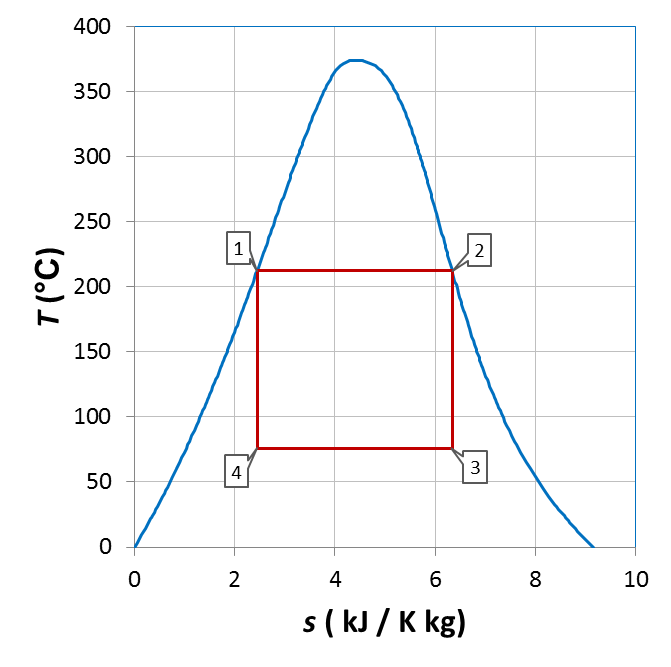
\includegraphics[width=0.5\textwidth]{./figures/Ts_q2.png}
\caption{$T$-$s$ diagram for a proposed Carnot cycle for a geothermal plant.}
\label{figure:q2}
\end{figure}

\begin{table}[h]
\caption{Values of thermodynamic properties of water/steam in the boiler and condenser}  % title of Table
\centering % used for centering table
\begin{tabular}{l l l l} % centered columns (4 columns)
\hline\hline %inserts double horizontal lines
 & Boiler & Condenser &  \\ [0.5ex] % inserts table
%heading
\hline % inserts single horizontal line
$P$ & 2000 & 40 & kPa \\ % inserting body of the table
$T$ & 212.4 & 75.9 & \SI{}{\celsius} \\
$h_f$ & 909 & 318 & \SI{}{\kilo\joule\per\kg} \\
$h_g$ & 2798 & 2636 & \SI{}{\kilo\joule\per\kg}  \\ [1ex] % [1ex] adds vertical space
\hline %inserts single line
\end{tabular}
\label{table:q2} % is used to refer this table in the text
\end{table}

\begin{enumerate}[label=\alph*)]
\item \lbrack\ 4 marks ]\ Drawing from the list of words below, describe the four processes that make up the cycle shown in Figure \ref{figure:q2}\par
\begin{table}[h]
\centering
\begin{tabular}{c c c c}
isothermal & constant & adiabatic & compression\\
boiler & condenser & pump & turbine \\
pressure & entropy & expansion&\\
\end{tabular}
\end{table}
\item \lbrack\ 1 mark ]\ In which process does heat $q_\mathrm{in}$ enter the working fluid?
\item \lbrack\ 1 mark ]\ What is the value of the specific heat input $q_\mathrm{in}$?
\item \lbrack\ 1 mark ]\ In which process is heat rejected by the working fluid?
\item \lbrack\ 1 mark ]\ In which process is work $w_\mathrm{out}$ done by the fluid?
\item \lbrack\ 2 marks ]\ Show that efficiency of this cycle is 28\%
\item \lbrack\ 2 marks ]\ What is the value of the specific work output $w_\mathrm{out}$?
\item \lbrack\ 2 marks ]\ What mass flow rate $\dot m$ of fluid would be required to achieve an output power of 1 MW?
\item \lbrack\ 1 mark ]\ How could the plant design be altered to achieve higher efficiency?
\item \lbrack\ 1 mark ]\ If the plant has low specific work output, in what way does that affect project costs?
\item \lbrack\ 2 marks ]\ Give two reasons why a Carnot cycle cannot be operated in practice.
\end{enumerate}

\begin{center}
\vspace{3cm}
--------- \textit{\middlewords} ---------
\end{center}
\newpage
\paragraph{\textbf{Question 3: (13 marks)}}
A geothermal power plant is proposed at a site where water can be brought to the surface at \SI{185}{\celsius} and where the only available heat sink is the ambient air at \SI{20}{\celsius}. An initial proposal is to use a water-steam plant, but this is rejected in favour of an Organic Rankine cycle using n-pentane, even though this has a lower efficiency.
$P$-$h$ and $T$-$s$ diagrams are shown for the two proposals in Figures \ref{figure:q3a} and \ref{figure:q3b} below.
\begin{figure}[h]
\centering
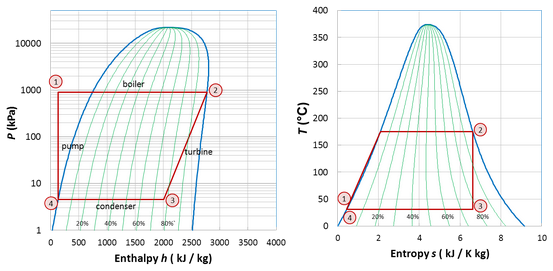
\includegraphics[width=0.85\textwidth]{./figures/steam-geo}
\caption{$P$-$h$ and $T$-$s$ diagrams for a proposed water-steam Rankine cycle for a geothermal plant.}
\label{figure:q3a}
\end{figure}
\begin{figure}[h]
\centering
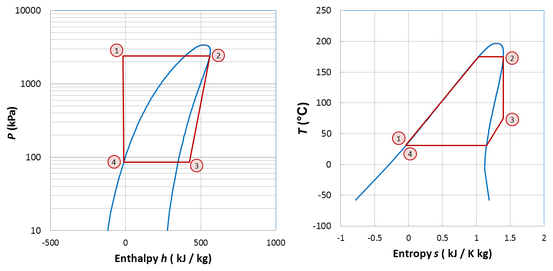
\includegraphics[width=0.85\textwidth]{./figures/ORC-geo}
\caption{$P$-$h$ and $T$-$s$ diagrams for a proposed Organic Rankine cycle for a geothermal plant.}
\label{figure:q3b}
\end{figure}

\begin{enumerate}[label=\alph*)]
\item \lbrack\ 2 marks ]\ Why have the plant designers not used a higher boiler pressure?
\item \lbrack\ 1 mark ]\ How can you tell from the $P$-$h$ diagrams of Figures \ref{figure:q3a} and \ref{figure:q3b} that the work input at the pumps is much less than the work output at the turbines?
\item \lbrack\ 3 marks ]\ Show that the efficiency of the water-steam plant is about 29\%.
\item \lbrack\ 2 marks ]\ What is the main operational reason for rejecting the water-steam cycle?
\item \lbrack\ 2 marks ]\ Why is a much higher mass flow rate of n-pentane required than would be required of water in the water-steam plant?
\item \lbrack\ 3 marks ]\  Name three desirable properties of refrigerant to be used in heat engines.

\end{enumerate}


\begin{center}
\vspace{3cm}
--------- \textit{\middlewords} ---------
\end{center}
\newpage

\paragraph{\textbf{Question 4: (14 marks)}}


A brine to water ground source heat pump (GSHP) using the vapour compression cycle is to be installed in a new house in central England, notionally at B0W35, with under-floor heating. The refrigerant R134a is to be used. The $P$-$h$ diagram for the cycle used is shown in Figure \ref{figure:q4a} on a date in the middle of summer.
\begin{figure}[h]
\centering
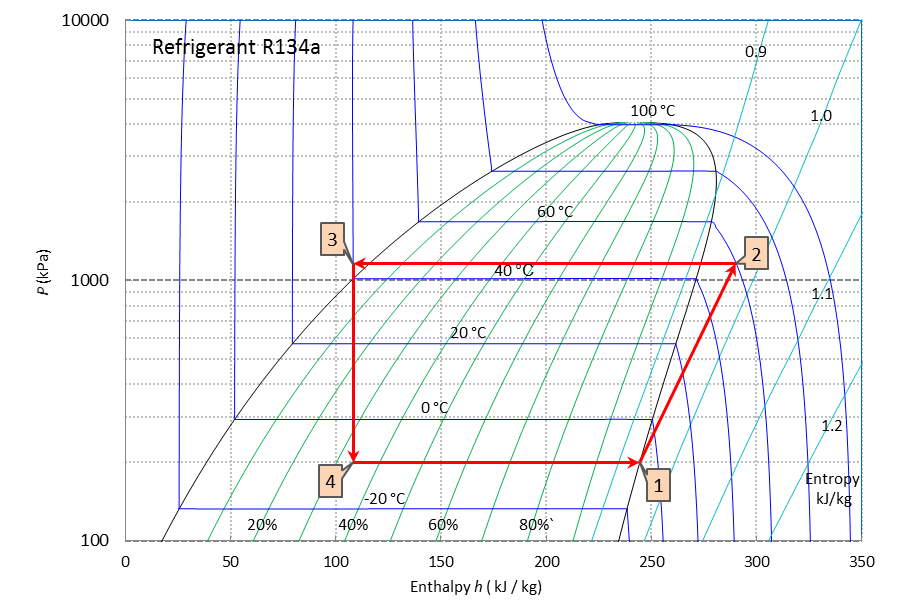
\includegraphics[width=0.85\textwidth]{./figures/B0W35}
\caption{$P$-$h$ diagram for a ground source heat pump operating between a brine temperature of \SI{0}{\celsius} and a radiator water temperature of \SI{35}{\celsius}}
\label{figure:q4a}
\end{figure}

\begin{enumerate} [label=\alph*)]
\item \lbrack\ 2 marks ]\ What is meant by the expression "B0W35"?
\item \lbrack\ 3 marks ]\ What is the coefficient of Performance (COP) of this heat pump?
\item \lbrack\ 2 marks ]\ How would the COP change if ordinarily sized radiators were used instead of under floor heating, assuming that the radiators provided sufficient heat to the house?
\item \lbrack\ 2 marks ]\ Explain why the COP would likely be lower in winter than in summer.
\item \lbrack\ 2marks ]\ How big does the COP need to be if the carbon dioxide emissions for space heating if using a gas boiler of efficiency 90\% are to be greater than those from using the heat pump for all space heating purposes? \par
Assume that the carbon intensity of UK electricity \SI{500}{\gram\per\kilowatthour} and that that of natural gas is \SI{200}{\gram\per\kilowatthour}.
\item \lbrack\ 3marks ]\ Justify the claim that heat pumps provide a sensible heating solution only in well insulated buildings.
\end{enumerate}
\begin{center}
\vspace{3cm}
--------- \textit{\lastwords} ---------
\end{center}


\label{finalpage}

%\begin{comment}

\newpage
\paragraph{\textbf{Solutions} \ }

\paragraph{\textbf{Solutions to Question 1: (17 marks)}}
There is a steady flow of heat upwards through the top few kilometres of the earth's crust.  The temperature at the surface in one location (A) is \SI{10}{\celsius} and the temperature at a depth of \SI{4}\km{} beneath the surface is \SI{106}{\celsius}. The rock in this location is granite with a thermal conductivity of $k=\SI{2.5}{\watt\per\celsius\per\metre}$
\begin{enumerate}[label=\alph*)]
\item \lbrack\ 2 marks ]\ Calculate the temperature gradient in the rocks beneath the surface.\par
$\dfrac{\Delta T}{x}=\dfrac{106-10}{4000}=\SI{0.024}{\celsius\per\metre}$
\item \lbrack\ 2 marks ]\ Show that the heat flow rate per square metre of ground is \SI{60}{\milli\watt\per\metre\squared}.\par
$\dot Q=k\dfrac{\Delta T}{x}=2.5\times 0.024 = \SI{60}{\milli\watt\per\metre\squared}$
\end{enumerate}
In another location (B)with the same surface temperature the same \SI{60}{\milli\watt\per\metre\squared} flows up through ground in which the granite is covered by a layer of clay \SI{1}{\kilo\metre} deep that has thermal conductivity $k=\SI{1.5}{\watt\per\celsius\per\metre}$
\begin{enumerate}[label=\alph*)]
\item \lbrack\ 3 marks ]\ Find the temperature at the base of the clay layer.\par
$\dfrac{\Delta T}{x}=\dfrac{\dot Q}{k}=\dfrac{0.06}{1.5}=\SI{0.04}{\celsius\per\metre}$\par
Hence\par
$\Delta T= 1000\times 0.04 = \SI{40}{\celsius}$\par
so that\par
$T_{1000}=T_0 + \Delta T = 10 + 40 = \SI{50}{\celsius}$\par
\item \lbrack\ 3 marks ]\ Find the depth at which the temperature reaches \SI{106}{\celsius} at this location\par
Need an additional $\Delta T$ in the granite layer of \SI{56}{\celsius} hence need an additional depth $x$ of\par
$x=\dfrac{k \Delta T}{\dot Q}=\dfrac{2.5\times 56}{0.06}=\SI{2333}{\metre}$\par
Hence depth at which temperature \SI{106}{\celsius} is now 1000 + 2333 = \SI{3333}{\metre}
\item \lbrack\ 3 marks ]\ Explain the advantages to a hot dry rocks geothermal energy scheme of finding a location such as B rather than A.\par
Higher temperatures now found nearer to the surface so drilling costs much reduced; also the impermeable nature of the clay will help keep the flowing water in the granite layer between the boreholes.
\item \lbrack\ 2 marks ]\ Why do many geothermal energy projects have a finite lifetime?\par
Heat extraction rate exceeds geothermal heat flux hence ground cools.\par
\item \lbrack\ 2 marks ]\ What proportion of the UK's energy needs might reasonably come from geothermal energy if the resource were fully and sustainably exploited?\par
About 1\%, or \SI{1}{\kilowatthour} per person per day.
\end{enumerate}


\paragraph{\textbf{Solutions to Question 2: (18 marks)}}
\begin{enumerate}[label=\alph*)]
\item \lbrack\ 4 marks ]\ Drawing from the list of words below, describe the four processes that make up the cycle shown in Figure \ref{figure:q2}\par
\begin{table}[h]
\centering
\begin{tabular}{c c c c}
isothermal & constant & adiabatic & compression\\
boiler & condenser & pump & turbine \\ 
pressure & entropy & expansion&\\
\end{tabular}
\end{table}
\par
1 to 2 : Constant pressure, isothermal expansion in the boiler\par
2 to 3 : Adiabatic expansion in the turbine\par
3 to 4 : Constant pressure, isothermal compression in the condenser\par
4 to 1 : Adiabatic compression in the pump.\par
\item \lbrack\ 1 mark ]\ In which process does heat $q_\mathrm{in}$ enter the working fluid?\par

In the boiler, 1 to 2
\item \lbrack\ 1 mark ]\ What is the value of the specific heat input $q_\mathrm{in}$?\par
$q_\mathrm{in}=h_g-h_f = 2798 - 909 = \SI{1889}{\kilo\joule\per\kg}$
\item \lbrack\ 1 mark ]\ In which process is heat rejected by the working fluid?\par
In the condenser 3 to 4
\item \lbrack\ 1 mark ]\ In which process is work $w_\mathrm{out}$ done by the fluid?\par
In the turbine 2 to 3
\item \lbrack\ 2 marks ]\ Show that efficiency of this cycle is 28\%\par
Cycle is reversible, hence\par $\eta=1-\frac{T_\mathrm{L}}{T_\mathrm{H}}=1-\frac{349}{486}=0.28$
\item \lbrack\ 2 marks ]\ What is the value of the specific work output $w_\mathrm{out}$?\par
$w=\eta\cdot q_\mathrm{in}=0.28\times 1889 = \SI{529}{\kilo\joule\per\kg}$
\item \lbrack\ 2 marks ]\ What mass flow rate $\dot m$ of fluid would be required to achieve an output power of 1 MW?\par
$\dot m =\frac{\dot w}{w}=\frac{\SI{1000}{\kilo\watt}}{\SI{529}{\kilo\joule\per\kg}}=\SI{1.9}{\kg\per\second}$
\item \lbrack\ 1 mark ]\ How could the plant design be altered to achieve higher efficiency?\par
Increase boiler pressure and hence boiler temperature
\item \lbrack\ 1 mark ]\ If the plant has low specific work output, in what way does that affect project costs?\par
Plant capital costs rise, since need more powerful pumps, larger pipes etc.
\item \lbrack\ 2 marks ]\ Give two reasons why this Carnot cycle cannot be operated in practice.\par
Mixed phase in turbine would damage turbine blades; hard to pump mixed phase; cannot easily stop condensation at precise dryness fraction required.
\end{enumerate}

\paragraph{\textbf{Solution to Question 3: (13 marks)}}
A geothermal power plant is proposed at a site where water can be brought to the surface at \SI{185}{\celsius} and where the only available heat sink is the ambient air at \SI{20}{\celsius}. An initial proposal is to use a water-steam plant, but this is rejected in favour of an Organic Rankine cycle using n-pentane, even though this has a lower efficiency.
$P$-$h$ and $T$-$s$ diagrams are shown for the two proposals in Figures \ref{figure:q3a} and \ref{figure:q3b} [below].


\begin{enumerate}[label=\alph*)]
\item \lbrack\ 2 marks ]\ Why have the plant designers not used a higher boiler pressure?\par
Boiler pressure is chosen to be whatever makes saturation temperature a few degrees below that of the heat source so that heat transfer will take place from the source to the boiler. In this geothermal plant, this temperature thus cannot be more than about 185-10=\SI{175}{\celsius}, and that sets the pressure. A higher boiler pressure would mean a saturation temperature higher than that of the geothermal water, and so cannot be used.
\item \lbrack\ 1 mark ]\ How can you tell from the $P$-$h$ diagrams of Figures \ref{figure:q3a} and \ref{figure:q3b} that the work input at the pumps is much less than the work output at the turbines?\par
Clearly a much smaller enthalpy change during the pumping  process.
\item \lbrack\ 3 marks ]\ Show that the efficiency of the water-steam plant is about 29\%.\par
Use enthalpy values from $P$-$h$ diagram.\par
$\eta=\dfrac{w_\mathrm{out}}{q_\mathrm{in}}=\dfrac{h_2-h_3}{h_2-h_1}=\dfrac{767}{2644}=0.29$
\item \lbrack\ 2 marks ]\ What is the main operational reason for rejecting the water-steam cycle?\par
Mixed phase in turbine - liquid will damage turbine blades, condenser pressure would have to be well below ambient so that air leaking in becomes a risk, and in pump-hard to pump vapour
\item \lbrack\ 2 marks ]\ Why is a much higher mass flow rate of n-pentane required than would be required of water in the water-steam plant?\par
Enthalpy change much smaller in turbine process, so specific work output much smaller, so flow rate needs to be higher for same output power - $\dot w=w\dot m$
\item \lbrack\ 3 marks ]\  Name three desirable properties of refrigerant to be used in heat engines.\par
Credit any three sensible suggestions: eg high heat capacity, thermal conductivity; chemically stable at temperatures and pressures required; zero ozone depletion potential; low GWP; non-toxic etc
\end{enumerate}

\paragraph{\textbf{Solution to Question 4: (14 marks)}}

A brine to water ground source heat pump (GSHP) using the vapour compression cycle is to be installed in a new house in central England, notionally at B0W35, with under-floor heating. The refrigerant R134a is to be used. The $P$-$h$ diagram for the cycle used is shown in Figure \ref{figure:q4a} on a date in the middle of summer.

\begin{enumerate} [label=\alph*)]
\item \lbrack\ 2 marks ]\ What is meant by the expression "B0W35"?\par
Underground brine loop at \SI{0}{\celsius} and radiator water loop at \SI{35}{\celsius}
\item \lbrack\ 3 marks ]\ What is the coefficient of Performance (COP) of this heat pump?\par
3.7 - from enthalpy differences found from $P$-$h$ diagram.
\item \lbrack\ 2 marks ]\ How would the COP change if ordinarily sized radiators were used instead of under floor heating, assuming that the radiators provided sufficient heat to the house?\par
Since smaller, radiators would need to be hotter for same heat output. Therefore COP would fall.
\item \lbrack\ 2 marks ]\ Explain why the COP would likely be lower in winter than in summer.\par
If ground is cooler, so is ground loop and therefore so is refrigerant in evaporator. Pressure in evaporator will therefore be lower, giving compressor more work to do to raise refrigerant pressure up to that of condenser. COP therefore falls. Also accept answer using sketches of cycle on $P$-$h$ diagram.
\item \lbrack\ 2marks ]\ How big does the COP need to be if the carbon dioxide emissions for space heating when using a gas boiler of efficiency 90\% are to be greater than those from using the heat pump for all space heating purposes? \par
Assume that the carbon intensity of UK electricity \SI{500}{\gram\per\kilowatthour} and that that of natural gas is \SI{200}{\gram\per\kilowatthour}.\par
Need $\mathrm{COP}\geq \dfrac{500}{200}\cdot0.9=2.25$

\item \lbrack\ 3 marks ]\ Justify the claim that heat pumps provide a sensible heating solution only in well insulated buildings.\par
COP needs to be high for the heat pump solution to deliver emissions and cost savings, due to the carbon intensity and cost differential between fossil fuels and electricity per unit of energy. (How high depends on fossil fuel being displaced, on current prices and on grid mix). For COP to be high, radiator temperatures need to be low, and thus radiators need to be oversized. In poorly insulated houses the size of radiator required, or even of floor space if UF heating used, would become unreasonable.
\end{enumerate}

%\end{comment}

\end{document}

